%==============================================================================
%  Weather and Climate Pattern Analysis
%  KOUAME Koffi Fidele, Data Analysis Internship
%==============================================================================
\documentclass[12pt,a4paper]{article}

\usepackage[T1]{fontenc}
\usepackage[utf8]{inputenc}
\usepackage{mathpazo}
\usepackage{microtype}

\usepackage[a4paper,top=2.5cm,bottom=2.4cm,left=2.6cm,right=2.6cm,
            headsep=14pt,footskip=26pt]{geometry}

\usepackage{graphicx}\graphicspath{{figures/}}
\usepackage{booktabs}\usepackage{array}\usepackage{tabularx}
\usepackage{enumitem}\usepackage{caption}\usepackage{fancyhdr}
\usepackage{titlesec}\usepackage{parskip}\usepackage{float}
\usepackage{xcolor}
\usepackage[section]{placeins}
\usepackage[hidelinks]{hyperref}

\definecolor{ink}{HTML}{111111}
\definecolor{rulegrey}{HTML}{9AA5B1}
\definecolor{soft}{HTML}{4A5560}
\definecolor{flag}{HTML}{A8641B}
\color{ink}

% Floats stay inside the section that discusses them, and LaTeX is allowed to
% pack more of them per page than the default permits.
\renewcommand{\topfraction}{0.92}
\renewcommand{\bottomfraction}{0.75}
\renewcommand{\textfraction}{0.06}
\renewcommand{\floatpagefraction}{0.80}
\setcounter{topnumber}{3}\setcounter{bottomnumber}{2}\setcounter{totalnumber}{4}
\setlength{\textfloatsep}{14pt plus 3pt minus 3pt}
\setlength{\intextsep}{13pt plus 3pt minus 3pt}
\widowpenalty=10000 \clubpenalty=10000

\titleformat{\section}{\normalfont\large\bfseries}{\thesection.}{0.6em}{}
\titleformat{\subsection}{\normalfont\normalsize\bfseries}{\thesubsection}{0.6em}{}
\titlespacing*{\section}{0pt}{18pt plus 4pt minus 3pt}{7pt}
\titlespacing*{\subsection}{0pt}{13pt plus 3pt minus 2pt}{4pt}

\captionsetup{font={normalsize,color=soft},labelfont={bf,color=ink},labelsep=period,
              justification=justified,singlelinecheck=false,skip=7pt}
\setlist[itemize]{leftmargin=1.25em,itemsep=3pt,topsep=4pt,parsep=0pt}
\setlist[enumerate]{leftmargin=1.5em,itemsep=4pt,topsep=4pt,parsep=0pt}

\pagestyle{fancy}\fancyhf{}
\fancyhead[L]{\footnotesize\color{soft}KOUAME Koffi Fidèle}
\fancyhead[R]{\footnotesize\color{soft}Weather and Climate Pattern Analysis}
\fancyfoot[C]{\footnotesize\color{soft}\thepage}
\renewcommand{\headrulewidth}{0.4pt}
\renewcommand{\headrule}{\color{rulegrey}\hrule height 0.4pt}

\newcommand{\F}[1]{\texttt{\small #1}}
\newcommand{\thinrule}{\textcolor{rulegrey}{\rule{\linewidth}{0.4pt}}}
\newcolumntype{L}{>{\raggedright\arraybackslash}X}
\newcommand{\PASS}{\textcolor{soft}{\textbf{correct}}}
\newcommand{\FAIL}{\textcolor{flag}{\textbf{incorrect}}}

\begin{document}

%==============================================================================
\begin{titlepage}
\centering
\vspace*{3.2cm}

{\large\scshape Data Analysis Internship}\\[2.4cm]

\thinrule\\[0.85cm]
{\LARGE\bfseries Weather and Climate Pattern Analysis}\\[0.55cm]
{\large A Ten-Year Daily Record, 2008 to 2017}\\[0.85cm]
\thinrule\\[1.1cm]

{\normalsize\color{soft}Data Quality \quad$\cdot$\quad Seasonality \quad$\cdot$\quad
Trend Testing \quad$\cdot$\quad Insights \quad$\cdot$\quad Power BI Dashboard}\\[3.4cm]

{\large\itshape Prepared by}\\[0.5cm]
{\Large\bfseries KOUAME Koffi Fidèle}\\[0.5cm]
{\normalsize\color{soft}koffifidelek59@gmail.com}\\[1.6cm]

{\large \today}
\vfill
\end{titlepage}

\tableofcontents
\newpage

%==============================================================================
\section{Executive summary}

The brief asks for a cleaned dataset, exploratory analysis, visualisations, an
interactive dashboard and clear insights. All five are delivered.

The file holds \textbf{3{,}271 daily observations} across 22 columns, from
1 February 2008 to 25 June 2017. It has \textbf{no missing cells and no duplicate
rows}, and every internal consistency rule passes. A routine audit would declare it
clean.

Three findings say otherwise, and none of them is visible to a missing-value count.

\textbf{First, nearly a third of the wind record is a placeholder.} The pair
\emph{west, 41 km/h} occurs on 1{,}027 days, 31.4\% of the file and 32 times the next
most frequent direction-and-speed combination. It covers every day of 2008 and 2009
and 80\% of 2010. Both values are legal in their columns, so no completeness or
validity check reaches it. Computed on the full file the prevailing wind appears
westerly on 43.6\% of days; on the 2{,}244 reliable days it is westerly on 17.7\%.

\textbf{Second, the record is not the calendar.} 162 days in the span carry no row at
all. A missing row leaves no trace in a missing-value count, because there is no cell
to be empty. Whole months are absent, and the observed-day count per calendar month
ranges from 240 to 310, a 29\% spread. Every monthly figure in this report is
therefore given twice, as a raw total and normalised per observed day, and a
conclusion is accepted only where the two agree.

\textbf{Third, the file cannot answer the spatial question.} The scenario describes
patterns across cities and countries. This file carries no city, country or station
column. It is a single-station daily record, so no spatial comparison is attempted.
What the file supports well is the temporal question: seasonality, extremes and trend.

The accompanying Power BI dashboard presents the indicators and the charts. Its six
indicator cards were verified against the data and are correct. Four statements in its
insight panel were written before this analysis was complete and do not match the
findings above; they are listed in section 8 and will be corrected in the next
revision.

\section{The data}

\begin{table}[htbp]\centering
\caption{The file as supplied}
\small
\begin{tabular}{@{}lr@{}}
\toprule
\textbf{Property} & \textbf{Value} \\
\midrule
Daily observations & 3{,}271 \\
Columns & 22 \\
First date & 2008-02-01 \\
Last date & 2017-06-25 \\
Calendar days in the span & 3{,}433 \\
\midrule
Missing cells & 0 \\
Duplicate rows & 0 \\
\textbf{Calendar days with no row} & \textbf{162 \enspace(4.7\%)} \\
\textbf{Location column} & \textbf{none} \\
\bottomrule
\end{tabular}
\end{table}

The measured quantities are the daily minimum and maximum temperature, rainfall,
evaporation, sunshine hours, wind gust direction and speed, wind speed and humidity
at 9\,am and 3\,pm, pressure at both hours, cloud cover in oktas at both hours, and
two derived rain flags.

\textbf{On the date format.} The \F{Date} column is text. Read as \F{m/d/Y} it parses
completely; read as \F{d/m/Y} it leaves 1{,}974 rows unparsed, which is 60\% of the
file. A single conversion call with the wrong assumption would discard those rows
without raising anything, so the format was tested rather than assumed.

%==============================================================================
\section{Data quality}

\begin{figure}[htbp]\centering
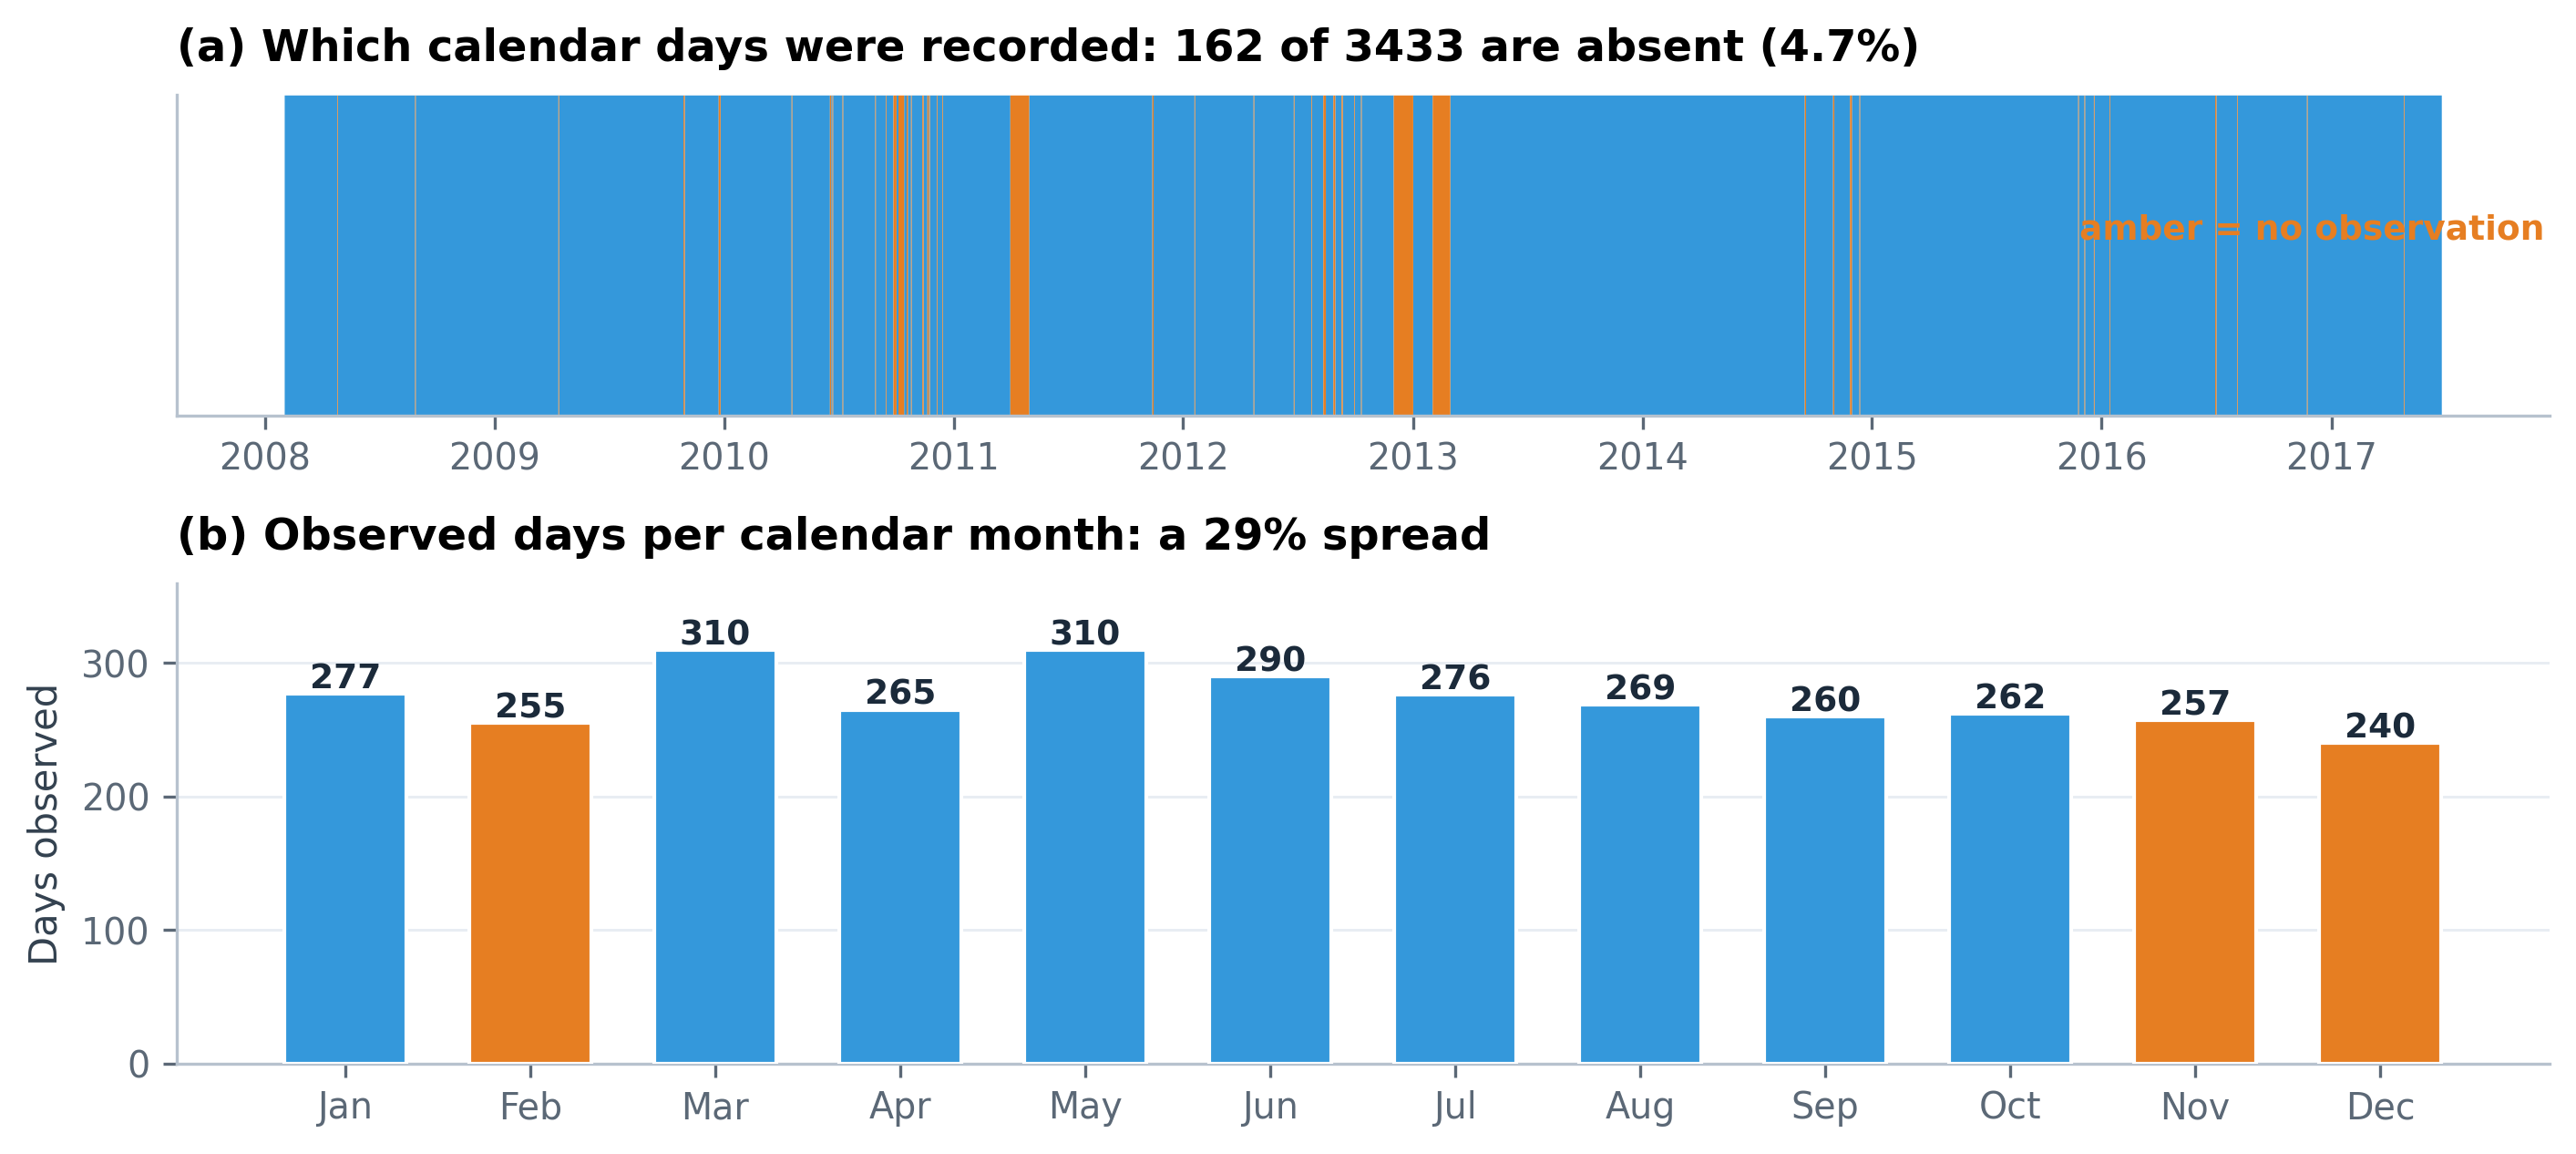
\includegraphics[width=0.96\linewidth]{01_coverage.png}
\caption{Calendar coverage. Panel (a) marks in amber every day of the span that
carries no observation; the three widest bands are whole months. Panel (b) shows the
consequence: the number of observed days differs by 29\% between the best and worst
covered calendar month, so a raw monthly total compares unequal samples.}
\end{figure}

\begin{table}[htbp]\centering
\caption{Consistency rules, all of which pass}
\small
\begin{tabular}{@{}lr@{}}
\toprule
\textbf{Rule} & \textbf{Breaches} \\
\midrule
Maximum temperature below minimum temperature & 0 \\
Humidity outside 0 to 100\% & 0 \\
Pressure outside 870 to 1085 hPa & 0 \\
Negative rainfall & 0 \\
Negative wind speed & 0 \\
\F{RainToday} disagrees with rainfall above 1 mm & 0 \\
\midrule
Cloud cover outside the 0 to 8 okta scale & \textbf{1} \\
\bottomrule
\end{tabular}
\end{table}

\textbf{On the single cloud value.} One record carries a cloud cover of 9. The okta
scale runs from 0, a clear sky, to 8, complete overcast. A value of 9 is used in some
archives as a code meaning the sky was obscured, by fog or by falling snow, which is
not the same as overcast. It was set to missing rather than to 8, because
substituting 8 would invent an observation that was never made.

\subsection{The constant-pair test}

A consistency rule cannot catch a value that is valid but invented. The test applied
here looks for a direction-and-speed pair that repeats more often than weather
allows. Wind gust is the natural candidate, because direction and speed come from one
instrument: when it fails, both are filled together.

\begin{table}[htbp]\centering
\caption{Share of each year carrying the pair \emph{west, 41 km/h}}
\small
\begin{tabular}{@{}lrrr@{}}
\toprule
\textbf{Year} & \textbf{Days observed} & \textbf{Carrying the pair} & \textbf{Share} \\
\midrule
2008 & 333 & 333 & \textbf{100.0\%} \\
2009 & 359 & 359 & \textbf{100.0\%} \\
2010 & 334 & 266 & \textbf{79.6\%} \\
2011 & 333 & 9 & 2.7\% \\
2012 & 320 & 8 & 2.5\% \\
2013 & 337 & 16 & 4.7\% \\
2014 & 357 & 4 & 1.1\% \\
2015 & 362 & 13 & 3.6\% \\
2016 & 361 & 18 & 5.0\% \\
2017 & 175 & 1 & 0.6\% \\
\midrule
\textbf{Total} & \textbf{3{,}271} & \textbf{1{,}027} & \textbf{31.4\%} \\
\bottomrule
\end{tabular}
\end{table}

The pattern is unambiguous. The pair is not scattered through the record as a
coincidence would be: it fills the first two years completely, fades through 2010 and
then all but disappears. This is a backfill of the period before the gust instrument
began reporting, and \textbf{wind gust is treated as unusable before 2011}
throughout this report.

\textbf{Why no other check finds it.} West is a legal direction and 41 km/h is a
legal speed, inside the observed range of 17 to 96. The cells are populated, so a
completeness audit sees nothing. The values are in range, so a validity rule sees
nothing. Only the improbable repetition of the exact pair gives it away.

\textbf{On \F{RainToday}.} The flag agrees with the rainfall column on all 3{,}271
rows. It is therefore derived from rainfall rather than independently recorded, and
it carries no information the rainfall column does not already hold.

%==============================================================================
\section{Cleaning}

\begin{table}[htbp]\centering
\caption{One decision per problem, with the reason for it}
\small
\begin{tabularx}{\linewidth}{@{}l r L@{}}
\toprule
\textbf{Item} & \textbf{Count} & \textbf{Decision and reason} \\
\midrule
Date format & 3{,}271 &
Parsed as \F{m/d/Y} after testing both conventions. The alternative discards 60\% of
the rows in silence. \\[3pt]
Cloud cover of 9 & 1 &
Set to missing, not to 8. The code means the sky was obscured, which is a different
observation from overcast. \\[3pt]
Absent calendar days & 162 &
\textbf{Not filled.} Interpolating a day's weather would invent 162 observations.
The gap is carried forward and every monthly figure is normalised for it instead. \\[3pt]
Seasons & all &
Southern-hemisphere convention: December to February is summer. The warmest month is
January and the coolest is July, so the northern convention would label the hottest
quarter winter and invert every seasonal conclusion. \\[3pt]
Incomplete years & 2 &
2012 has 320 observed days and 2017 stops in June with 175. Both are excluded from
year-on-year comparison and kept for everything else. \\
\bottomrule
\end{tabularx}
\end{table}

Nine derived measures are added: the daily mean temperature, the diurnal range, mean
humidity, mean wind speed, mean pressure, mean cloud, the calendar fields, and the
season. \textbf{No row was deleted}; 22 columns become 35.

%==============================================================================
\section{Indicators}

\begin{table}[htbp]\centering
\caption{The record in eleven figures}
\small
\begin{tabular}{@{}lr@{}}
\toprule
Observations & 3{,}271 days \\
Mean temperature & 18.94 \textdegree C \\
Highest temperature & 45.80 \textdegree C \\
Lowest temperature & 4.30 \textdegree C \\
Mean humidity & 61.47\% \\
Mean wind speed & 17.19 km/h \\
Strongest gust & 96 km/h \\
Total rainfall & 10{,}932 mm \\
Rainy days & 849 \enspace(26.0\% of days) \\
Mean pressure & 1017.2 hPa \\
Mean sunshine & 7.17 hours \\
\bottomrule
\end{tabular}
\end{table}

\begin{table}[htbp]\centering
\caption{The five extremes in the record}
\small
\begin{tabular}{@{}llr@{}}
\toprule
\textbf{Event} & \textbf{Date} & \textbf{Value} \\
\midrule
Hottest day & 2013-01-18 & 45.8 \textdegree C \\
Coldest day & 2010-06-30 & 4.3 \textdegree C \\
Wettest day & 2015-04-21 & 119.4 mm \\
Strongest gust & 2014-06-28 & 96 km/h \\
Most humid day & 2011-10-20 & 100\% \\
\bottomrule
\end{tabular}
\end{table}

%==============================================================================
\section{Patterns}

\subsection{The seasonal cycle}

\begin{figure}[htbp]\centering
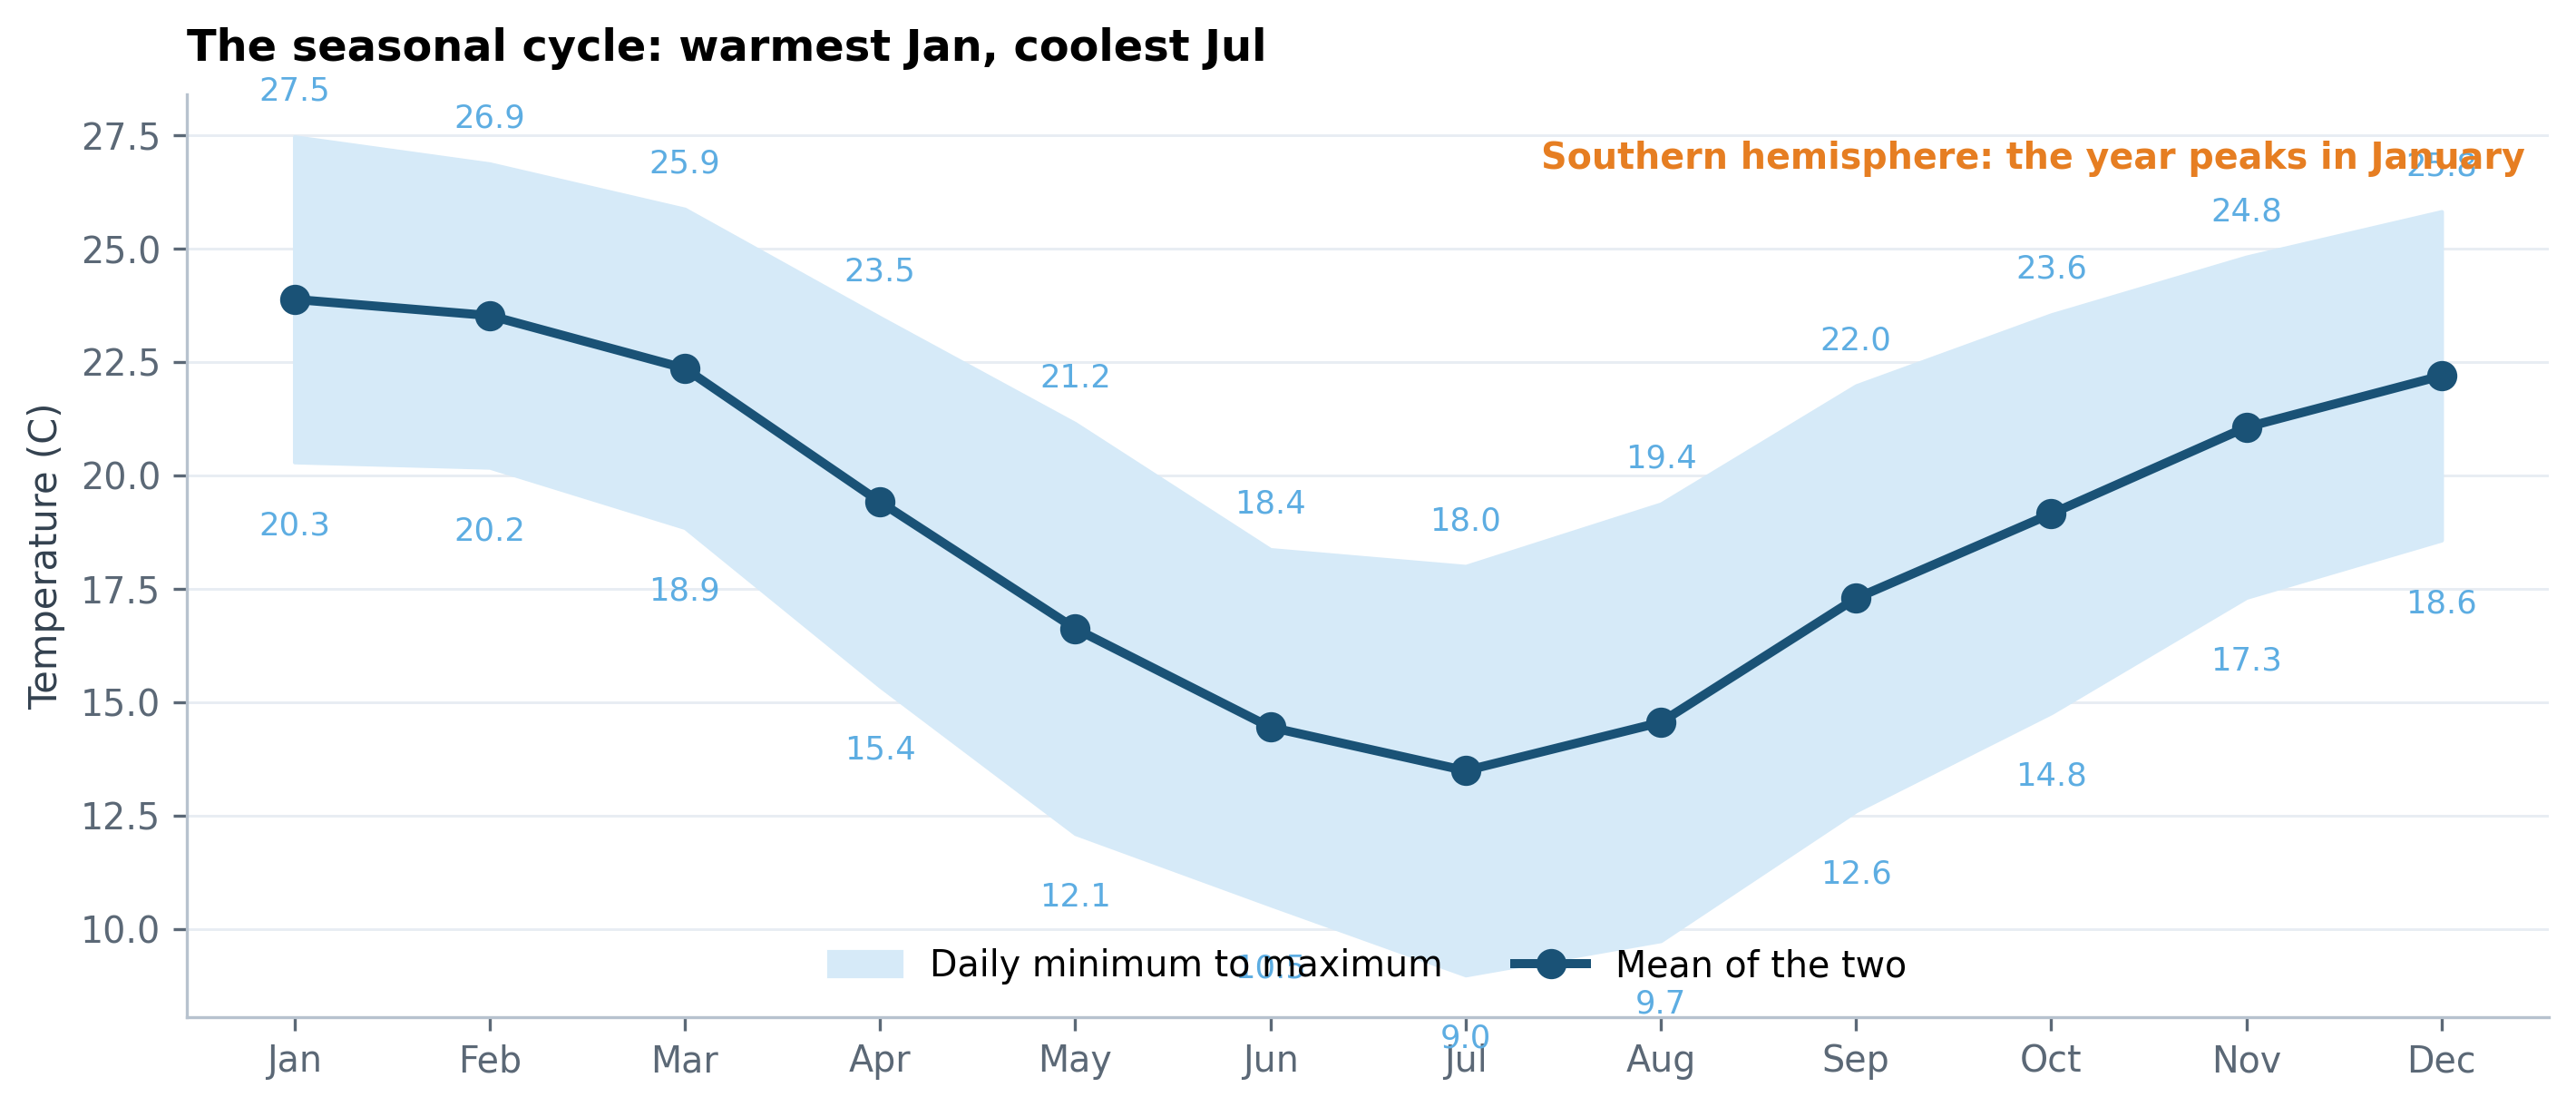
\includegraphics[width=0.94\linewidth]{02_temperature_cycle.png}
\caption{The annual temperature cycle. The band spans the mean daily minimum to the
mean daily maximum; the line is the mean of the two. The year peaks in January and
troughs in July, which is the southern-hemisphere signature and the reason the
seasonal convention was set accordingly.}
\end{figure}

\begin{table}[htbp]\centering
\caption{The four seasons, southern-hemisphere convention}
\small
\begin{tabular}{@{}lrrrr@{}}
\toprule
\textbf{Season} & \textbf{Days} & \textbf{Mean temp} & \textbf{Rain per day} & \textbf{Humidity} \\
\midrule
Summer (Dec to Feb) & 772 & 23.25 \textdegree C & 3.31 mm & 63.8\% \\
Autumn (Mar to May) & 885 & 19.48 \textdegree C & 4.00 mm & 64.4\% \\
Winter (Jun to Aug) & 835 & 14.18 \textdegree C & 3.63 mm & 60.5\% \\
Spring (Sep to Nov) & 779 & 19.17 \textdegree C & 2.31 mm & 56.8\% \\
\bottomrule
\end{tabular}
\end{table}

\subsection{Rainfall}

\begin{figure}[htbp]\centering
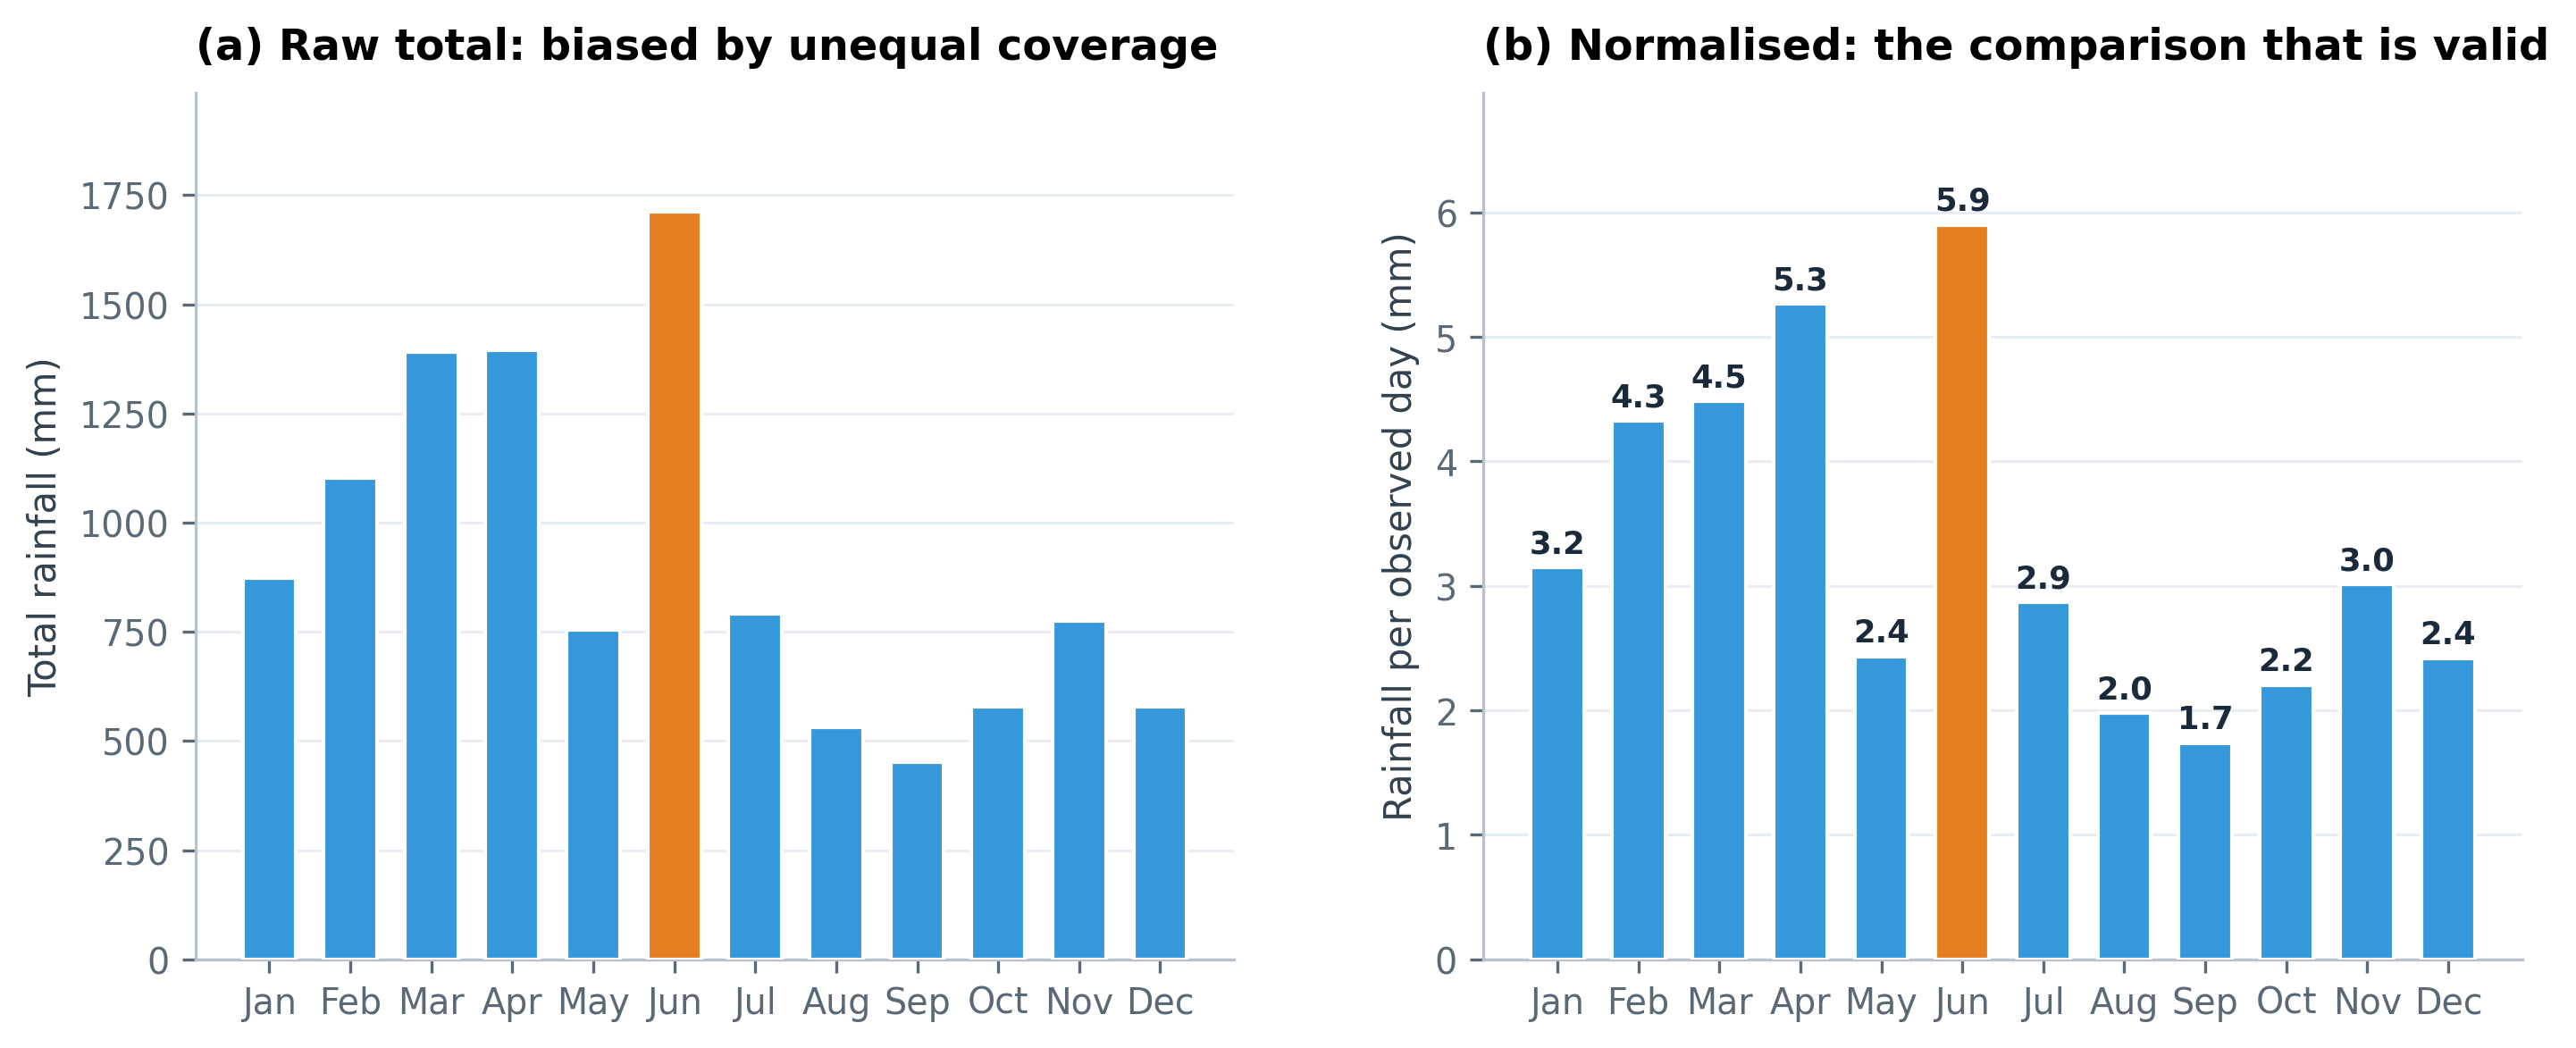
\includegraphics[width=0.96\linewidth]{03_rainfall.png}
\caption{Rainfall by calendar month, ranked two ways. Panel (a) is the raw total,
which compares months observed for different numbers of days. Panel (b) divides by
the observed days and is the comparison that is valid. The two rankings agree, so
June is genuinely the wettest month and September the driest; the agreement is the
evidence, not an assumption.}
\end{figure}

June receives 5.90 mm per observed day against 1.73 mm in September, a factor of 3.4.
Autumn is the wettest season at 4.00 mm per day, and spring the driest at 2.31 mm.

\subsection{Wind}

\begin{figure}[htbp]\centering
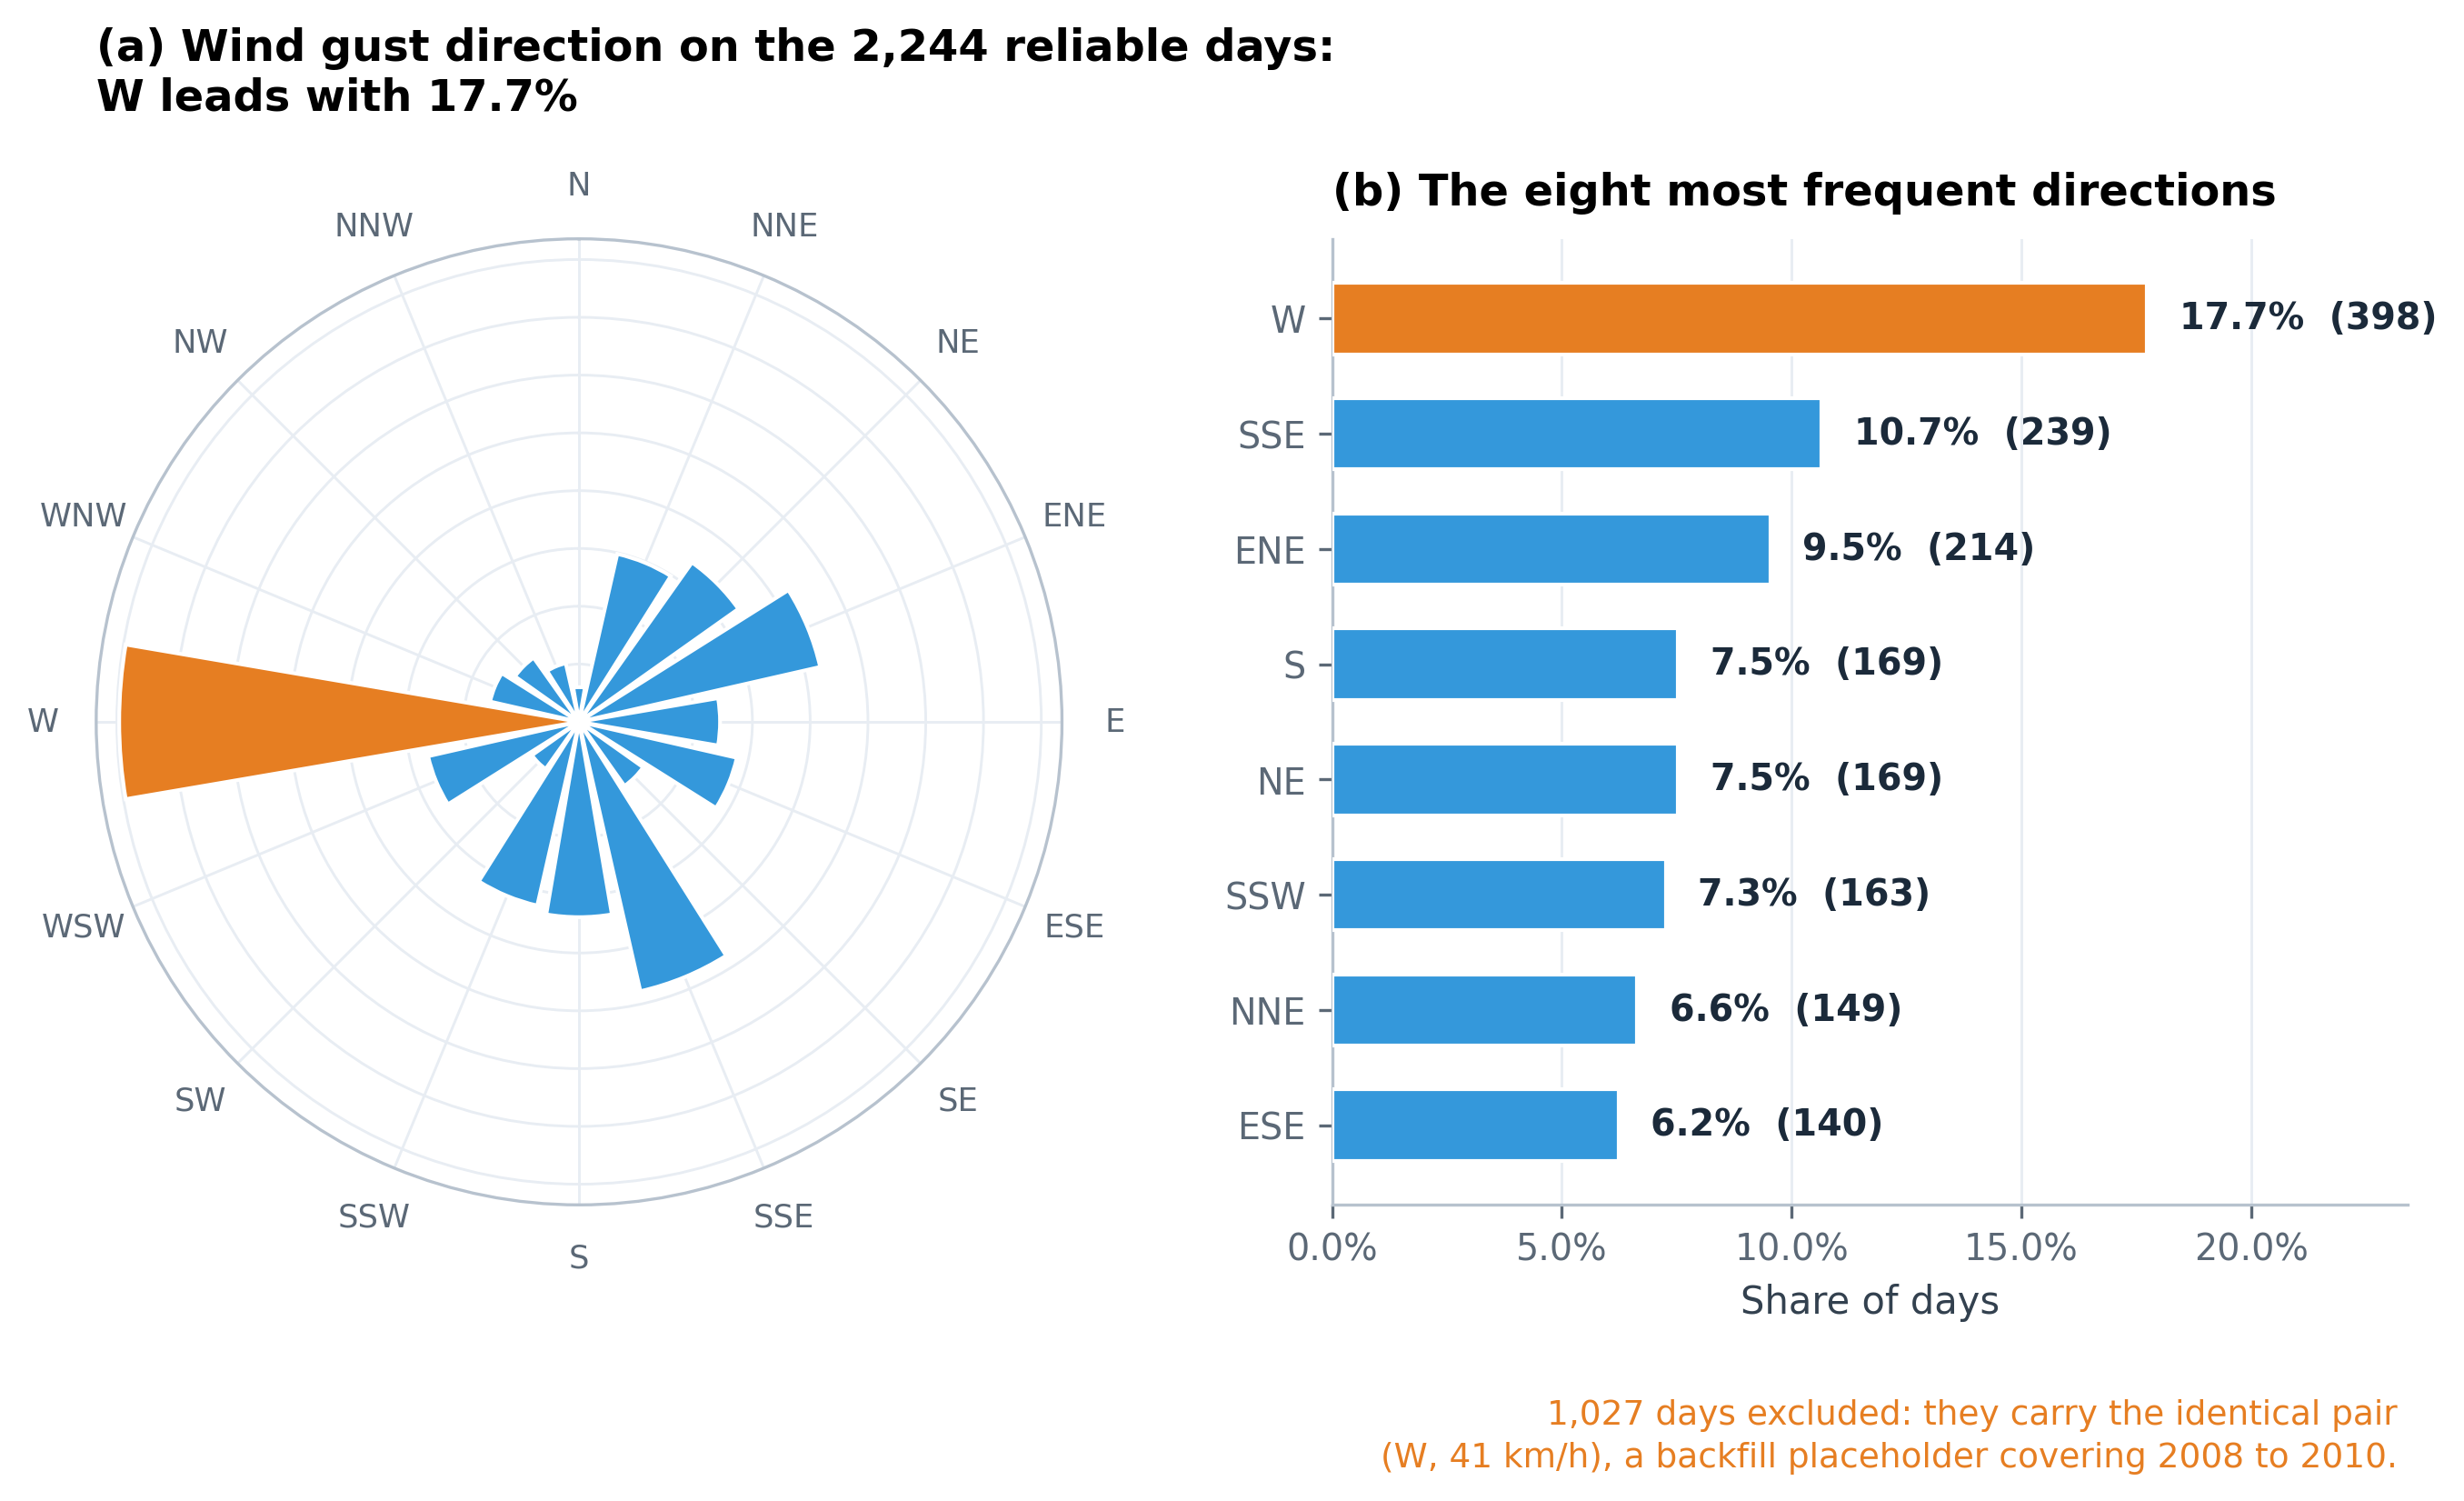
\includegraphics[width=0.86\linewidth]{04_wind_rose.png}
\caption{Wind gust direction, computed on the 2{,}244 reliable days. West leads with
17.7\%, ahead of south-south-east at 10.7\%. The 1{,}027 placeholder days are
excluded: including them returns 43.6\% for west, which is the backfill speaking
rather than the site.}
\end{figure}

\subsection{Trend}

\begin{figure}[htbp]\centering
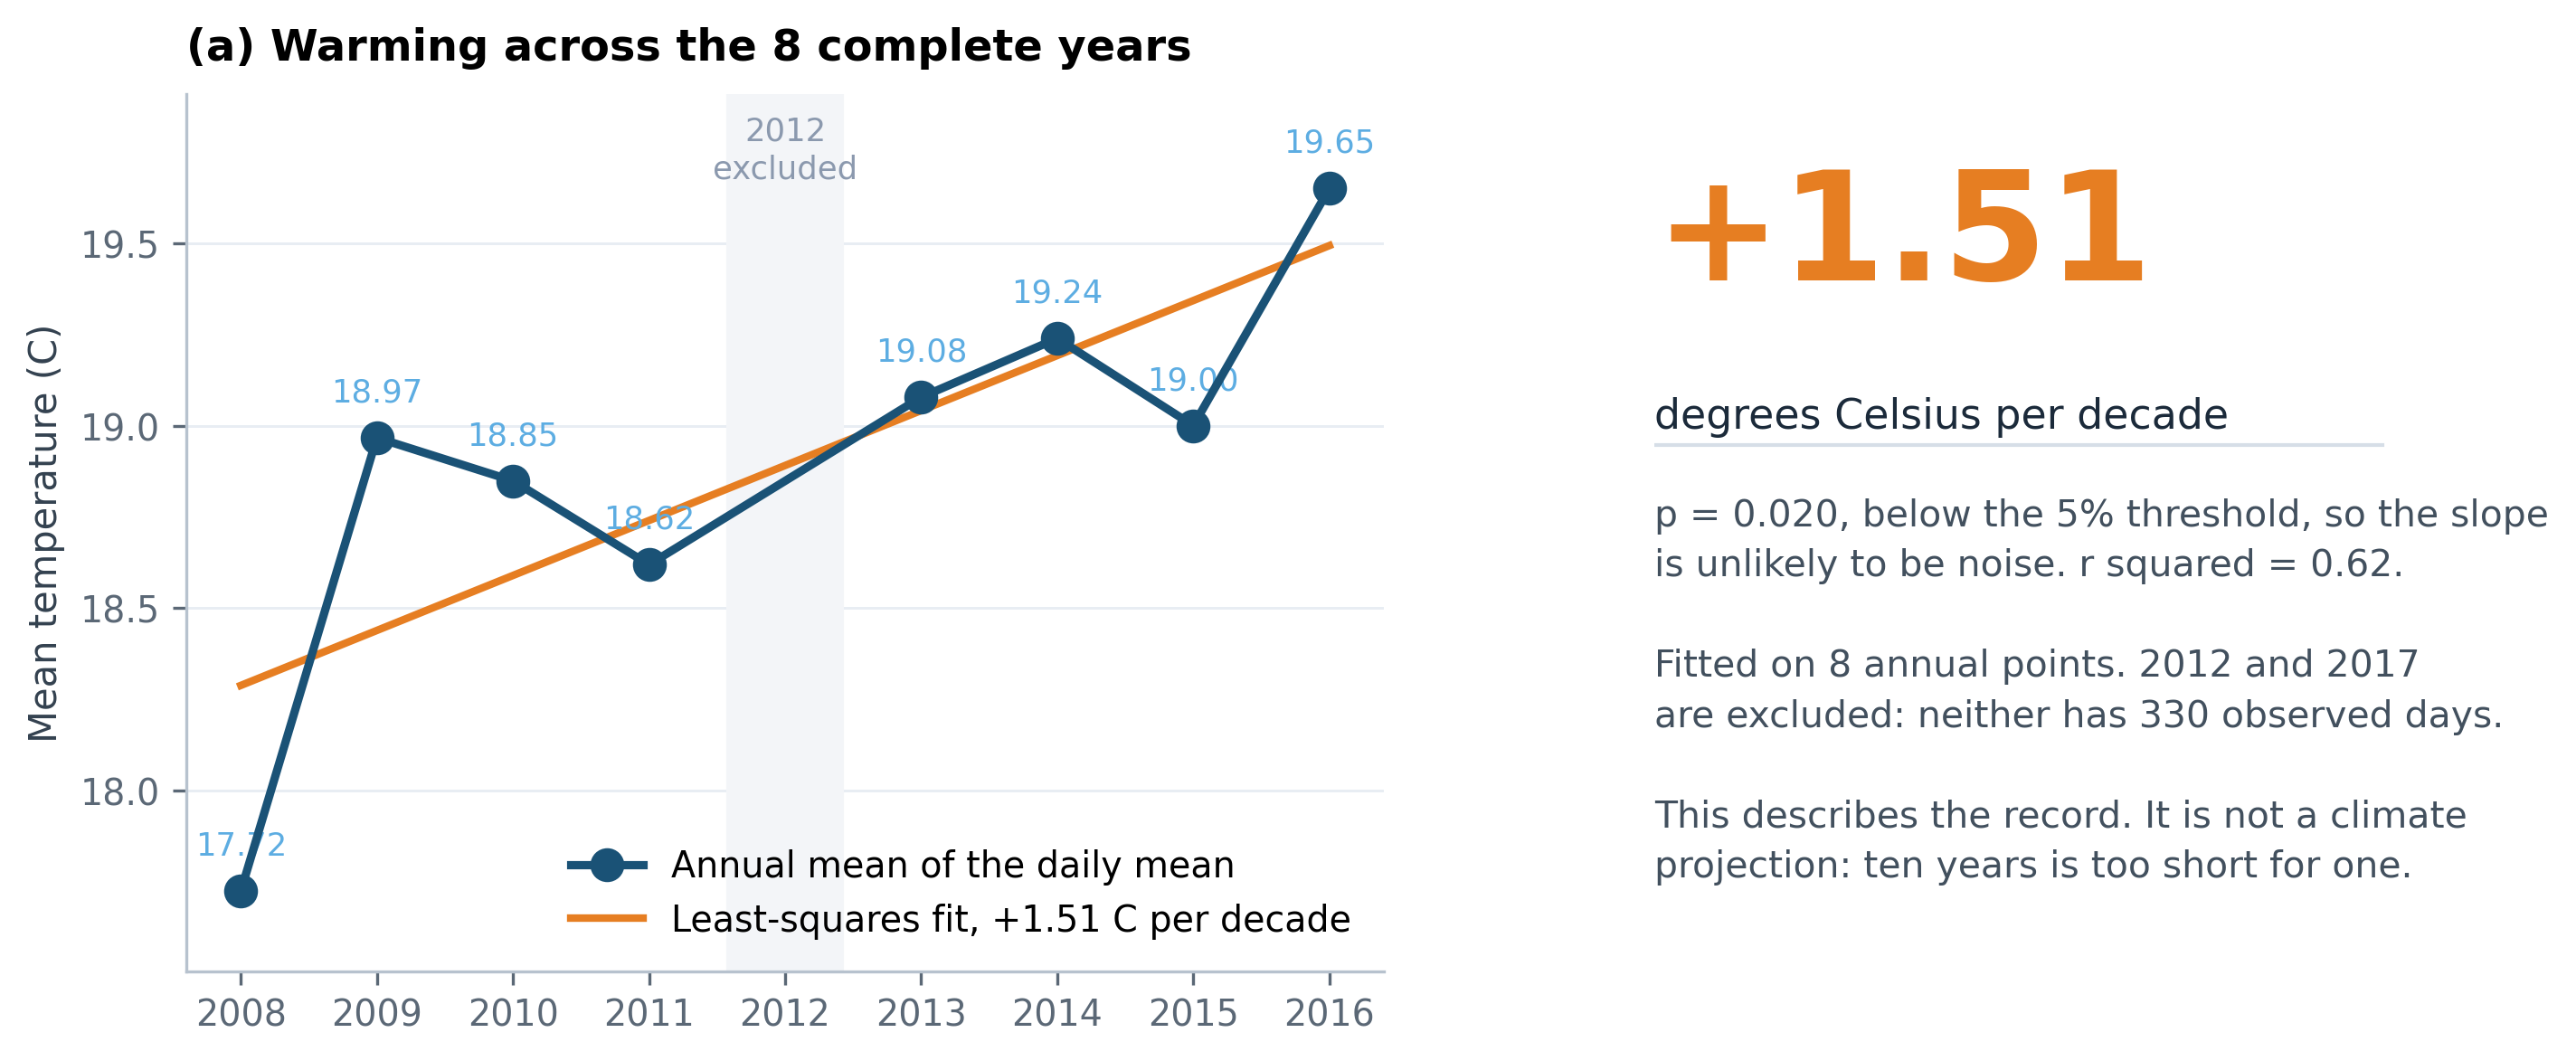
\includegraphics[width=0.94\linewidth]{05_trend.png}
\caption{The warming trend, tested rather than asserted. The slope is
$+1.51$ \textdegree C per decade with $p = 0.020$, which is significant at the 5\%
level. The interval is nonetheless short, and the caption on the right states what
the number does and does not support.}
\end{figure}

\subsection{What moves with what}

\begin{figure}[htbp]\centering
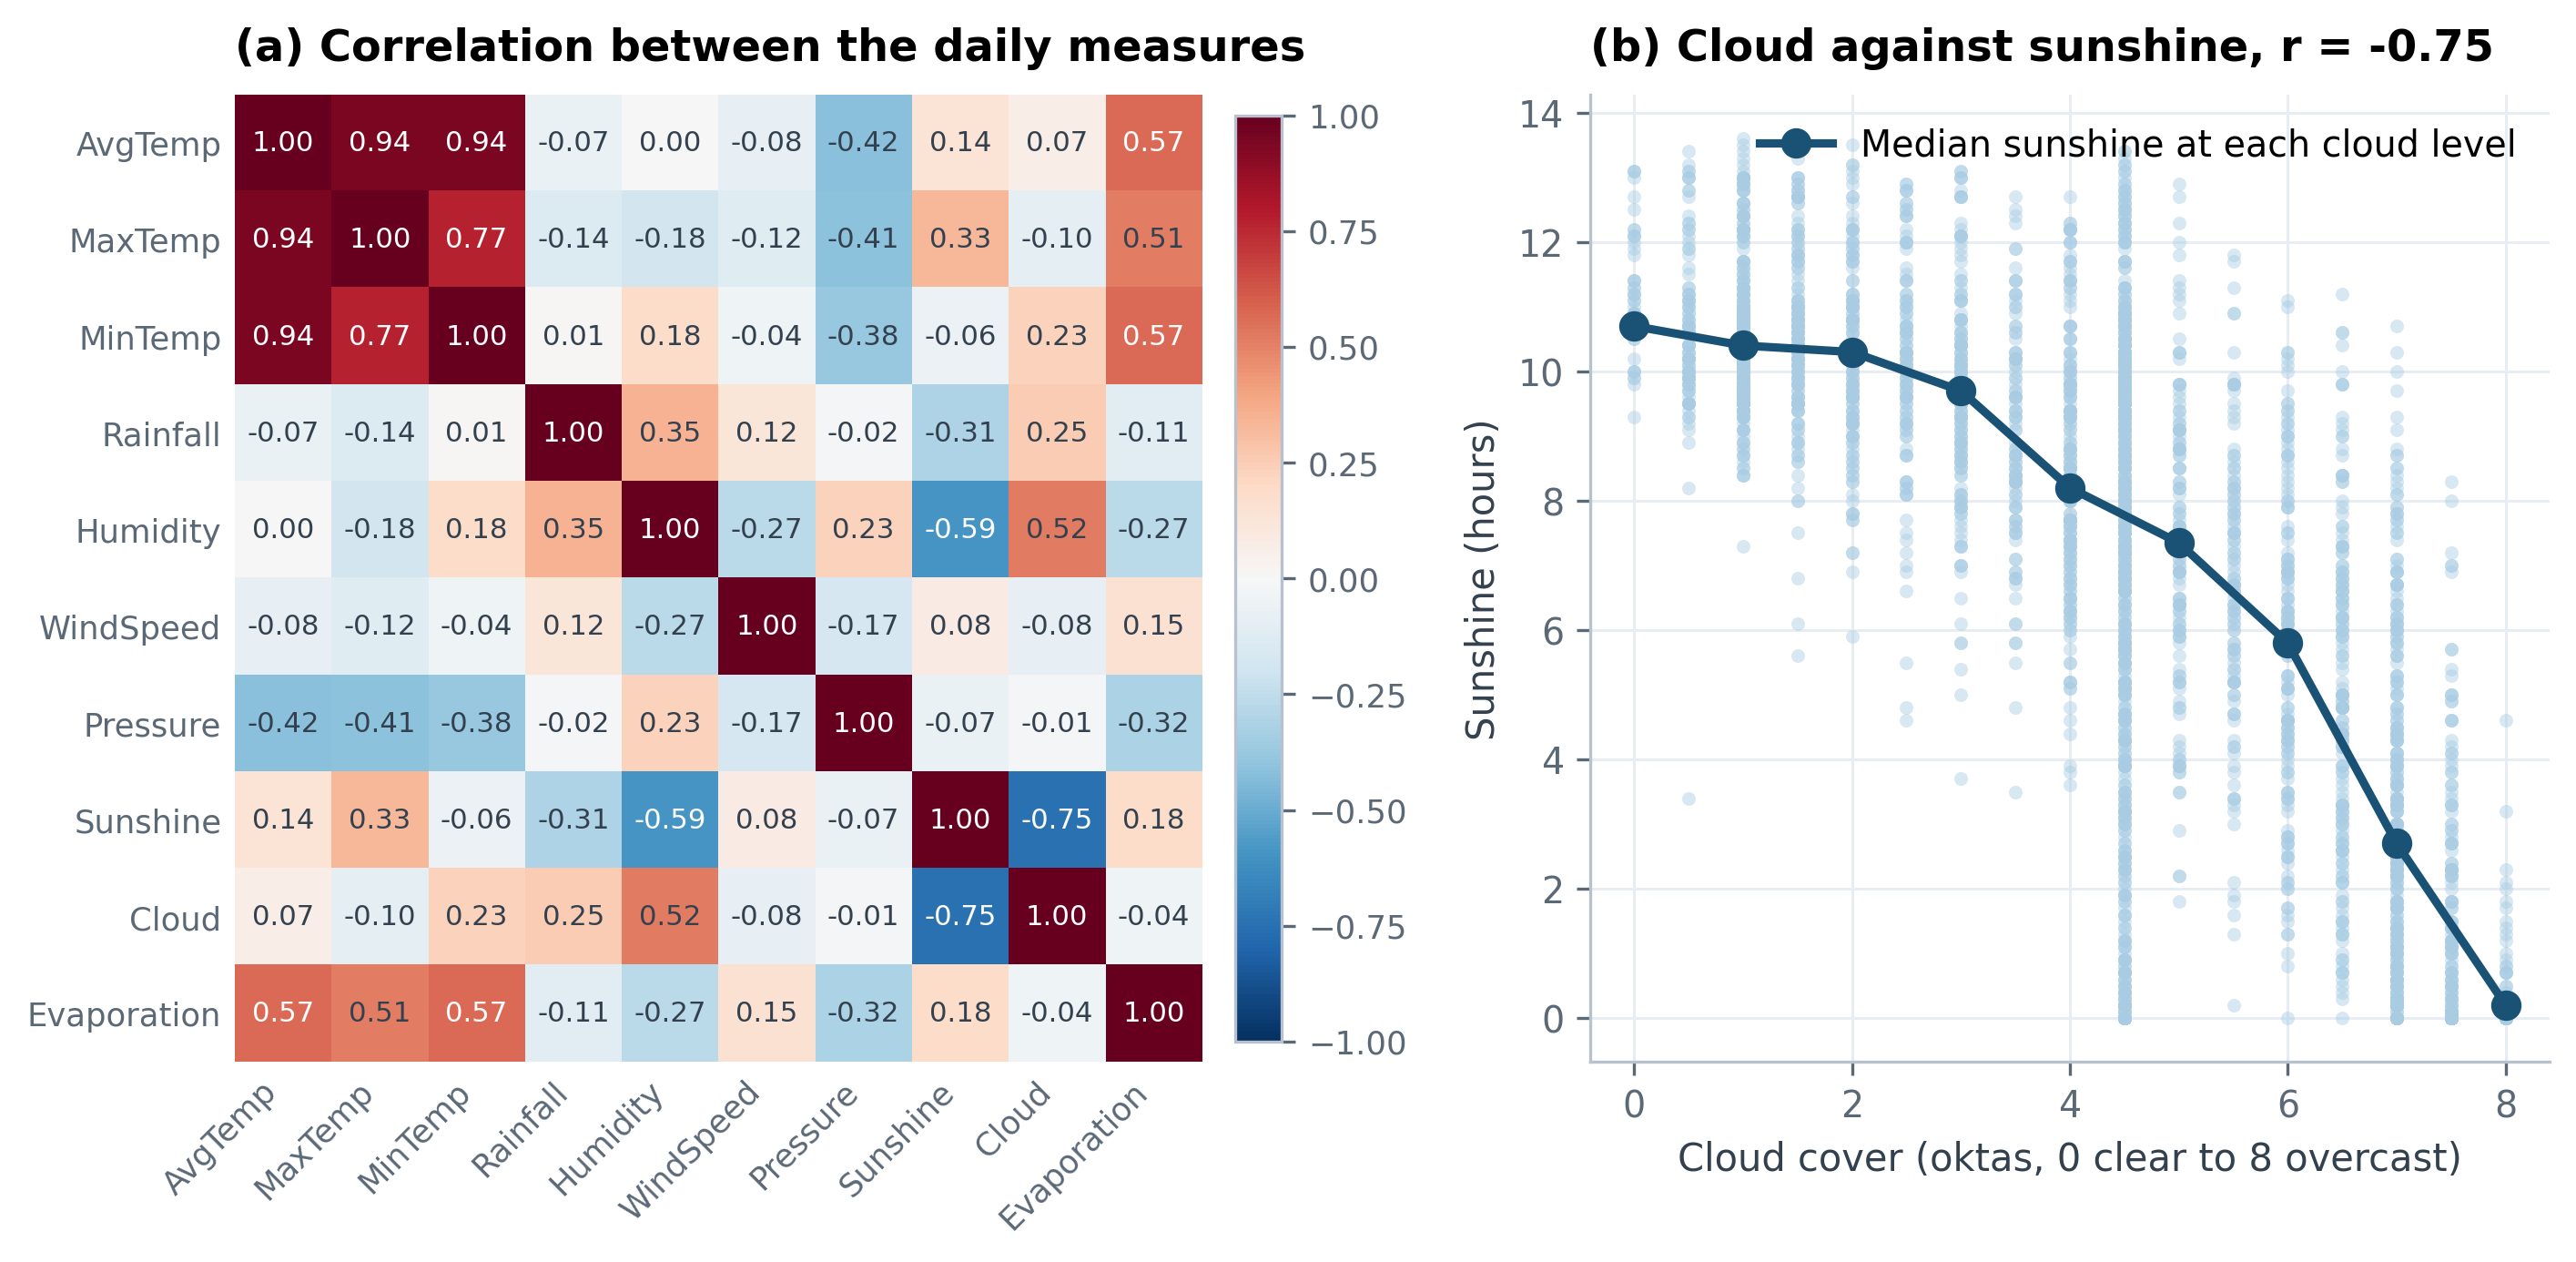
\includegraphics[width=0.94\linewidth]{06_relationships.png}
\caption{Relationships between the daily measures. The strongest association that is
not mechanical is cloud cover against sunshine at $r = -0.75$: the two measure the
same physical state from opposite directions. Temperature against evaporation at
$+0.57$ is the strongest relationship between genuinely distinct quantities.}
\end{figure}

%==============================================================================
\section{Insights}

\subsection{The record is not the calendar}

162 calendar days carry no row, and whole months are absent. A monthly total
therefore compares samples of unequal size, with a 29\% spread between the best and
worst covered month.

Here the correction does not change the ranking: June is the wettest month and
September the driest on both the raw total and the per-day rate. \textbf{That is a
result, not a formality.} It was established by computing both, and it means the
seasonal conclusion can be stated with confidence rather than hope.

\textbf{Recommendation.} Publish rainfall as millimetres per observed day alongside
the total, and show the observed-day count beside any monthly figure.

\subsection{The seasonal signal is southern hemisphere}

The warmest month is January and the coolest is July. Applying the northern
convention would place the hottest quarter in winter and invert every seasonal
statement in the study. The dashboard's humidity insight is exactly this error:
humidity peaks in February, and February was read as winter.

\textbf{Recommendation.} State the hemisphere convention on the dashboard itself. It
costs one line and removes an entire class of misreading.

\subsection{Warming of 1.51 degrees per decade}

The trend across the eight complete years is $+1.51$ \textdegree C per decade with
$p = 0.020$ and $r^2 = 0.62$. The slope is unlikely to be noise.

It is also fitted on eight annual points spanning nine years. A decade is short for a
climate statement, and a single station cannot speak for a region.

\textbf{Recommendation.} Report the slope with its p-value and its sample size, never
the slope alone. Describe it as a property of this record, not as a projection.

\subsection{Rain and warmth are in opposition}

Autumn delivers 4.00 mm per observed day and winter 3.63, against 2.31 in spring.
June alone receives 3.4 times what September receives. The wet season and the warm
season are in opposition, which is the single most useful fact in the record for
anyone planning around it.

\subsection{Cloud and sunshine measure the same state}

Cloud cover and sunshine hours correlate at $-0.75$. They describe the same physical
state from opposite directions, so a model using both gains little from the second.
The strongest relationship between genuinely distinct quantities is temperature
against evaporation at $+0.57$.

\textbf{Recommendation.} Keep one of the pair in any predictive work, and prefer
sunshine, which is measured on a continuous scale rather than in eight steps.

%==============================================================================
\section{The Power BI dashboard}

The dashboard presents the indicators, the seasonal profiles, the wind rose and the
correlation panel on a single page.

It is cross-filtered throughout: selecting a month in the rainfall panel, a direction
in the wind rose or a point in the correlation scatter filters every other visual at
once, and the three slicers for year, month and season do the same. Every figure
quoted in this report is the whole-record value, obtained with no selection active.

\begin{figure}[htbp]\centering
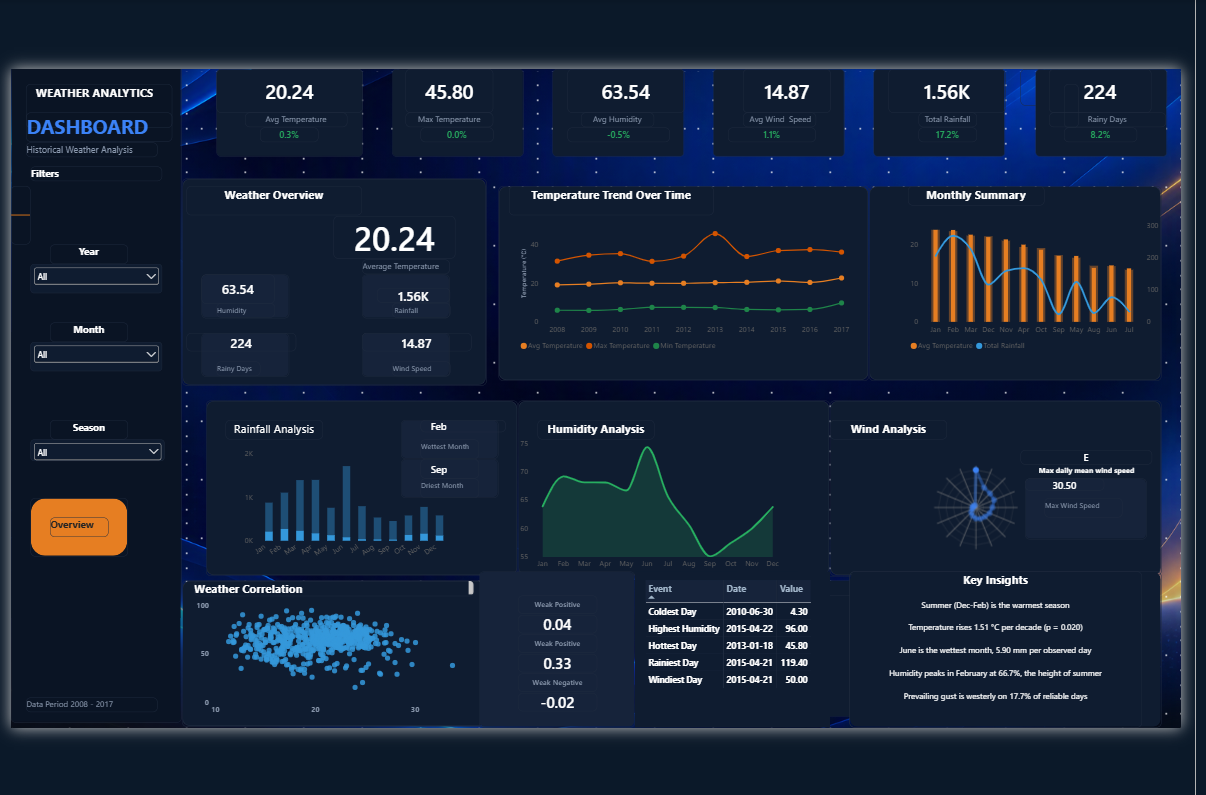
\includegraphics[width=0.98\linewidth]{07_powerbi_dashboard.png}
\caption{The Weather Analytics dashboard. Six indicator cards across the top, the
temperature trend and monthly summary in the middle band, and the rainfall, humidity
and wind panels below, with the key insights at the lower right. The capture was taken
with a cross-filter selection active, which is why the cards read 20.24 \textdegree C
and 224 rainy days rather than the whole-record values of 18.94 and 849 quoted in
section 5: selecting any element filters every other visual on the page. The slicers
for year, month and season work the same way.}
\end{figure}

\FloatBarrier

\section{Limitations and work in hand}

\subsection{What the data cannot support}

\textbf{No location.} The file has no city, country or station column, so the spatial
comparison the brief describes cannot be performed. Everything reported here
describes one station.

\textbf{Wind before 2011.} 1{,}027 days carry the placeholder pair, including all of
2008 and 2009. Every wind figure in this report excludes them, and the exclusion is
stated wherever a wind number appears.

\textbf{162 absent days}, clustered in 2010 to 2013 and removing whole months. Any
figure not normalised for observed days is biased by them.

\textbf{Eight years for a trend.} The warming slope is statistically significant and
still rests on eight annual points at one station. It describes this record and is not
a climate projection.

\textbf{\F{RainToday} is derived.} It agrees with the rainfall column on every row, so
it is not an independent observation and should not be treated as one.

\textbf{Correlation, not causation.} Nothing here establishes why the measures covary.

\subsection{Corrections identified for the next dashboard revision}

The insight panel of the dashboard was written before the analysis in sections 3 and 6
was complete. Four of its statements do not match the findings, and each has a
straightforward fix.

\begin{table}[htbp]\centering
\caption{Items identified during this analysis, to be applied in the next revision}
\small
\begin{tabularx}{\linewidth}{@{}l L@{}}
\toprule
\textbf{Item} & \textbf{Correction} \\
\midrule
Rainy Days card shows 1K &
The count is 849. The card applies a thousands abbreviation to a three-digit number,
which rounds up by 18\%. Set the display unit to None. \\[3pt]
``February recorded the highest rainfall'' &
June is the wettest month on both rankings, 5.90 mm per observed day against 4.32 in
February. The Rainfall Analysis panel on the same page already shows June, so the two
will be brought into agreement. \\[3pt]
``Humidity peaks during winter months'' &
Humidity peaks in February at 66.7\% and is lowest in September at 53.3\%. February is
summer under the southern-hemisphere convention established in section 4. \\[3pt]
``Dominant wind direction: SE'' &
West leads with 17.7\% on the reliable days; south-east accounts for 4.5\%. The Wind
Analysis panel displays E separately, and both will be recomputed on the reliable
subset once the placeholder flag is added to the model. \\
\bottomrule
\end{tabularx}
\end{table}

Two statements on the page are confirmed by the analysis and need no change: summer is
the warmest season, and the temperature trend is upward. The report quantifies the
second at $+1.51$ \textdegree C per decade, which the dashboard can now state rather
than imply.

\textbf{The underlying cause of three of the four.} The placeholder in the wind record
and the hemisphere convention were both established in this report, after the
dashboard was built. Adding the reliability flag and the season field to the Power BI
model resolves the wind and humidity items together.

\section*{Deliverables}
\addcontentsline{toc}{section}{Deliverables}

\begin{table}[H]\centering
\small
\begin{tabular}{@{}ll@{}}
\toprule
\textbf{File} & \textbf{Content} \\
\midrule
\texttt{Weather\_Analysis.ipynb} & Commented notebook, executed \\
\texttt{report.pdf} & The present report \\
\texttt{INSIGHTS.md} & Insights and recommendations \\
\texttt{data/weather\_clean.csv} & Cleaned dataset, 3{,}271 rows \\
\texttt{analysis.py} & The code, commented \\
\texttt{figures/} & Six analysis figures \\
\texttt{Weather\_Dashboard.pbix} & The Power BI dashboard \\
\bottomrule
\end{tabular}
\end{table}

\vfill
\noindent\thinrule\\[4pt]
{\small\textbf{KOUAME Koffi Fidèle}\quad\textcolor{soft}{$\cdot$}\quad
\color{soft}Data Analysis Internship\quad$\cdot$\quad koffifidelek59@gmail.com}

\end{document}
